\documentclass[main.tex]{subfiles}

\begin{document}

\chapter{Examined systems}\label{ch:examined_systems}

\section{Silicon}\label{sec:systems_silicon}

Silicon is the fundamental material in modern transistors and as such is one of the pillars of the digital revolution.
Analogue to the Stone, Bronze or Iron Age, the current age of civilization can thus be called the Silicon Age \cite{chabal_fundamental_2001}.
Consequently, silicon is a well studied material from an experimental and theoretical standpoint.
Combining this with the fact that \acrshort{dft} calculations on silicon are not particularly expensive makes it an ideal system for an introduction to \acrshort{dft} calculations as well as a good benchmarking system.
Consequently, all benchmarks in this thesis were run on silicon first and with the information gained from that, benchmarks on a more expensive system were run.

The calculations in \cref{ch:optimisation_scf} and \ref{ch:optimization_ph} were made with a plane-wave cutoff of \(\SI{70}{\rydberg}\) and on a \(40\times40\times40\)/\(6\times6\times6\) \(k\)-point grid respectively.
All calculations use a PBE (Perdew-Burke-Ernzerhof \cite{perdew_generalized_1996}) XC-functional with a norm-conserving \acrshort{pp} generated using Vanderbilt's method \cite{hamann_erratum_2017}.

\section{\TaS}\label{sec:systems_tas2}

Tantalum Disulfide (\TaS) belongs to the class of \acrfull{tmdc}s.
The most common stoichiometry of compounds in this class is MX\textsubscript{2}, where M is a transition-metal and X is a chalcogen atom.
\acrshort{tmdc}s occur with different atomic coordinations.
Fig. \ref{fig:tas2_structure} shows the structure of trigonal-prismatic \TaS (2H-\TaS), which consists of a hexagonal transition-metal lattice between two hexagonal chalcogen lattices whose atoms are aligned on top of each other.
Seen from above, they form a honeycomb lattice.

\begin{figure}
    \begin{subfigure}{0.49\textwidth}
        \centering
        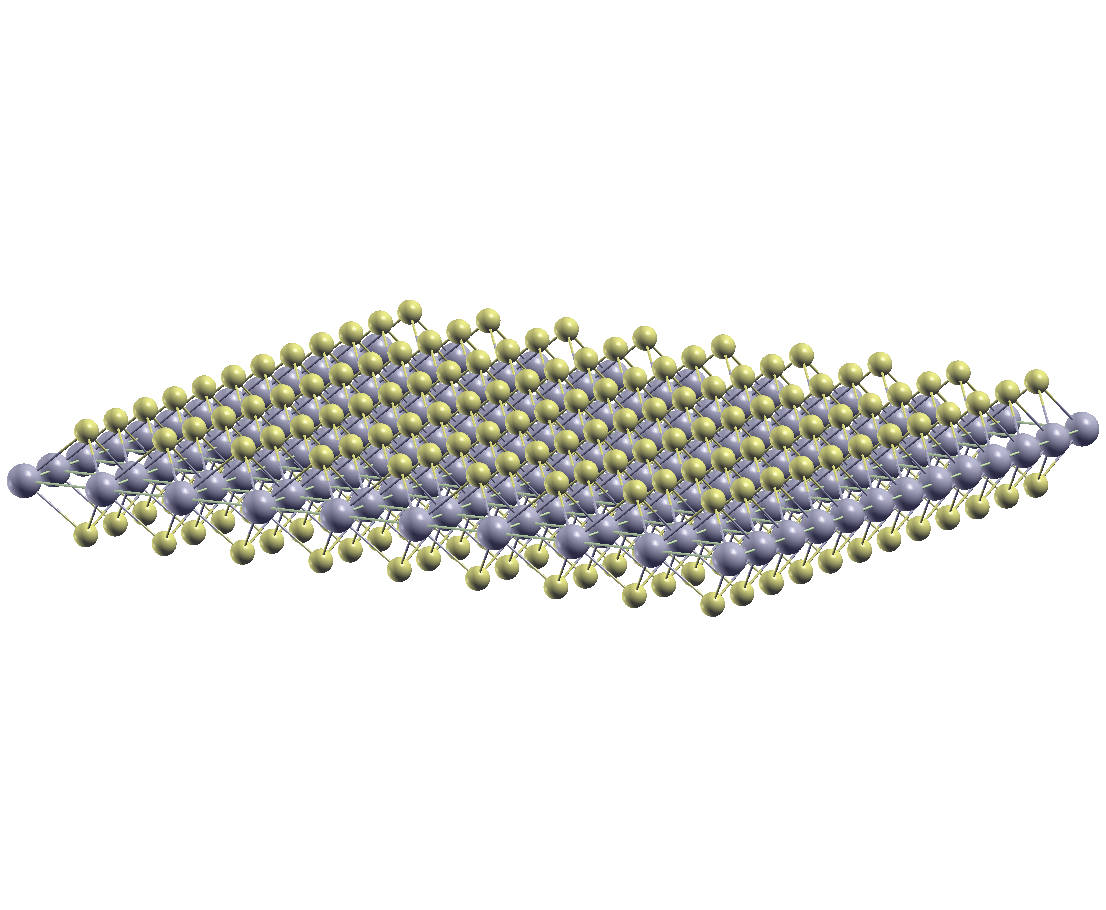
\includegraphics[width=\textwidth]{structure_images/TaS2_from_the_side.png}
    \end{subfigure}
    \begin{subfigure}{0.49\textwidth}
        \centering
        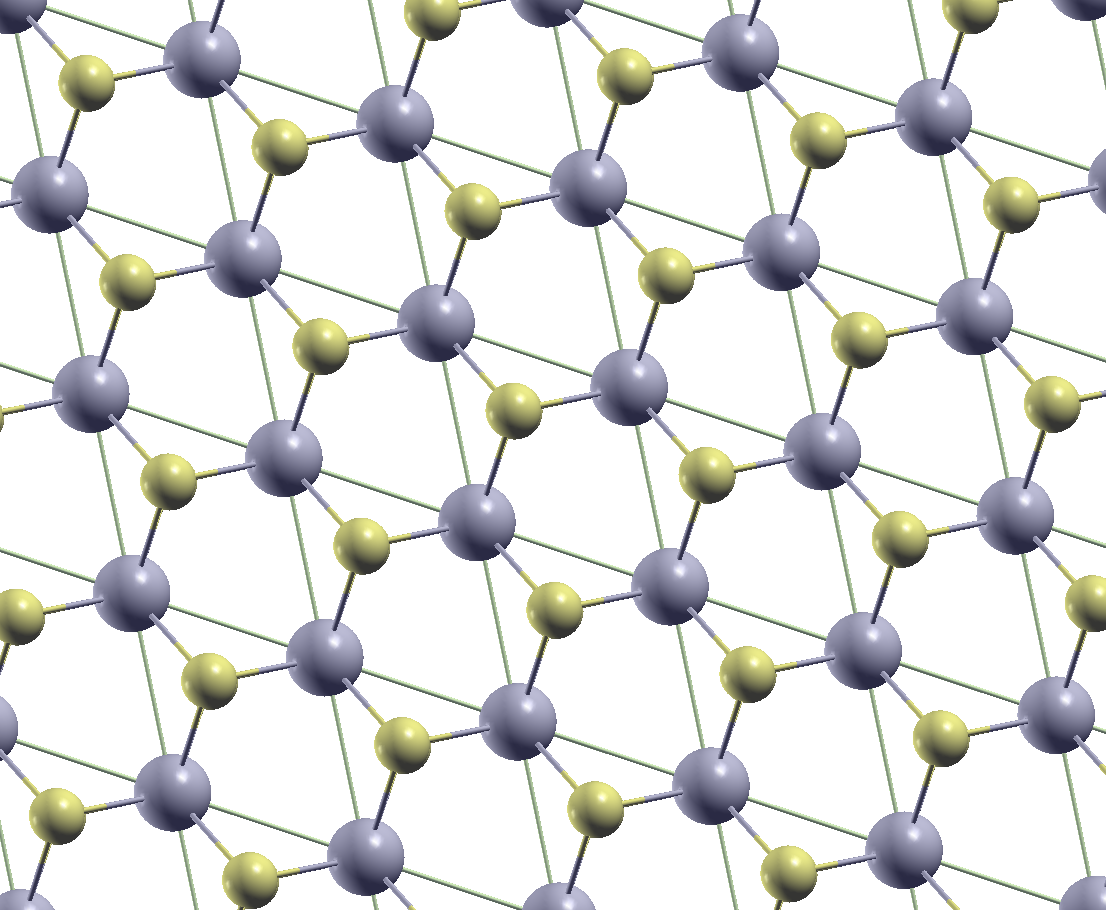
\includegraphics[width=\textwidth]{structure_images/TaS2_from_above.png}
    \end{subfigure}
    \caption{Crystal structure of a 2H-\TaS monolayer as seen from the side (left) and from the top (right). Visualized using XCrySDen \cite{kokalj_xcrysdennew_1999}}
    \label{fig:tas2_structure}
\end{figure}

\acrshort{tmdc}'s were known and studied as a bulk material since more than five decades \cite{wilson_transition_1969}.
The more recent possibility to do experiments on freestanding monolayers \cite{novoselov_two-dimensional_2005} has brought these materials back into focus,  as bulk \TaS shows superconductivity and formation of charge density waves, so the effect of the reduction of dimensionality on these phenomenon can be studied on them \cite{navarro-moratalla_enhanced_2016}.

\subsection{Charge-density waves}

A charge density wave is a periodic modulation of the electronic charge density of a solid.
This changes the potential acting on the nuclei, so a distortion of the lattice accompanies the formation of a charge-density wave, to the point where both terms are used interchangeably.
Fig. \ref{fig:tas2_cdw_structure} shows a charge-density wave in 2H-\TaS.
\TaS forms charge-density waves in both the bulk case \cite{wilson_charge-density_1974} and as a monolayer \cite{hall_environmental_2019}.

A simple model for the formation of charge-density waves in a one-dimensional case was given by Peierls in 1955.
Following the review by Grüner \cite{gruner_dynamics_1988}, the argument is as follows: 
the formation of a periodic distortion of the lattice creates a unit cell twice as large as the original one, so the Brillouin zone becomes half as large.
Thus, the bands fold back onto this smaller Brillouin zone and split due to an avoided crossing.
This results in a gap at the Fermi level.

\begin{figure}[h]
    \centering
    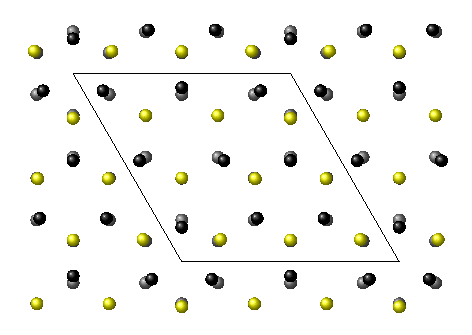
\includegraphics[width=0.5\textwidth]{symmetric.pdf}
    \caption{\TaS charge density wave. Gray dots are atoms in the symmetric phase, yellow/black dots are the Tantalum/Sulfur atoms in the charge density wave phase.}
    \label{fig:tas2_cdw_structure}
\end{figure}


\subsection{Computational parameters}

All calculations on the 2H-\TaS charge-density wave were made with a plane-wave cutoff of \(\SI{100}{\rydberg}\) and on a \(12\times12\) \(k\)-point grid.
The calculations use a PBE XC-functional with a norm-conserving \acrshort{pp} generated by Hartwigsen et al. \cite{hartwigsen_relativistic_1998}.
Input files for both the symmetric and charge density wave phase were kindly provided by Dr.\,Jan Berges.

\end{document}
